\documentclass{report}

\usepackage{graphicx} % Required for inserting images
\usepackage{amsmath,amssymb}
\usepackage[ruled,vlined]{algorithm2e}

\usepackage{url}

\usepackage{pgfplots}
\pgfplotsset{compat=1.18} % Use a recent compatibility version
\usetikzlibrary{arrows.meta} % For nicer arrows



\definecolor{maincolor}{HTML}{1E90FF}

\usepackage[colorlinks=true,
            urlcolor=maincolor]{hyperref}

\usepackage{xcolor}
\usepackage{listings}




\begin{document}

\section{Stream}

Il prossimo algoritmo che vedremo è quello degli \textbf{Stream}.  
Prima di parlarne, però, dobbiamo capire cosa sono i \textbf{Pseudo-Random Number Generator}, perché sono la base degli stream, anche se inizialmente possono sembrare non avere nulla a che fare con essi.

\subsection{PRNG}

Per chi ha già creato qualche programma in \textbf{C}/\textbf{C++}, può darsi che abbia dovuto \textbf{generare dei numeri casuali}.  
Tuttavia, è difficile crearli perché i computer sono sistemi \textbf{deterministici}, cioè ad ogni input corrisponde sempre lo stesso output.  
Quindi, per i computer è impossibile generare numeri realmente casuali; per questo motivo sono stati inventati gli \textbf{Pseudo-Random Number Generator}, ovvero dei generatori di numeri \textbf{pseudo-casuali}, che a noi \textbf{sembrano} casuali, ma che in realtà sono deterministici.


Un primo esempio è il \textbf{Linear Congruential Generator} (\textit{LCG}), che parte da alcuni valori iniziali $X_0$, $a$, $c$ e $m$ ($X_0$ è detto \textbf{seme} o \textbf{seed}), i quali possono essere scelti a piacere.  
A partire da questi valori, possiamo generare nuovi numeri pseudo-casuali con la seguente formula:


\begin{equation*}
    X_{n+1} = aX_n + c \pmod{m}
\end{equation*}

Per chi non lo sapesse, il simbolo $\pmod{n}$ indica il \textbf{resto della divisione} tra due numeri.  
Per esempio, $9 \pmod{4}$ significa che devo fare la divisione $9/4$ e considerare solo il resto.  
In questo caso, $9/4 = 2$ con resto $1$, quindi $9 \pmod{4} = 1$.  
Riprenderemo questi concetti nei capitoli dedicati a \textbf{RSA} e \textbf{Diffie-Hellman}.


Per esempio, se scegliamo come valori iniziali $m = 9$, $a = 4$, $c = 1$ e come seme $X_0 = 3$, otteniamo la seguente sequenza di numeri pseudo-casuali:


\begin{align*}
    %X_1 &= 4 \cdot X_0 + 1 \pmod{9} \\
    X_1 &= 4 \cdot 3 + 1 \pmod{9} \\
        &= 13 \pmod{9} \\
    X_1  &= 4
    \\
    \\
    X_2 &= 4 \cdot X_1 + 1 \pmod{9} \\
        &= 4 \cdot 4 + 1 \pmod{9} \\
        &= 17 \pmod{9} \\
    X_2 &= 8 
    \\
    \\
    X_3 &= 4 \cdot 8 + 1 \pmod{9} \\
        &= 33 \pmod{9} \\
    X_3 &= 6
\end{align*}

Per questa configurazione, i primi valori generati dalla sequenza sono:

\begin{equation*}
    4, 8, 6, 7 ,2, 1, 5, 3, 4 ... 
\end{equation*}

Si nota che, all'apparenza, sembra una sequenza casuale di numeri, ma in realtà deriva da una formula e da alcune variabili fissate inizialmente ($a$, $m$, $c$ e $X_0$).

Un problema di questi generatori è che sono \textbf{ciclici}, nel senso che, prima o poi, la sequenza si ripete.  
Per esempio, se continuiamo la sequenza di prima:


\begin{equation*}
    \underline{4, 8, 6}, 7, 2, 0, 1, 5, 3, \underline{4, 8, 6}, 7, 2, 0, 1, 5, 3, \underline{4, 8}
\end{equation*}


Notiamo che questa sequenza è lunga 8 numeri, perché poi si ripete.  
Questo problema è dovuto al fatto che abbiamo scelto numeri \textbf{piccoli}; se invece scegliamo numeri più grandi, ad esempio a 10 o 15 cifre, la ciclicità sarà molto più ampia.


Questo sistema di generazione, però, ha un altro problema: dati alcuni output, è possibile ricavare i parametri ($a$, $m$ e $c$).  
Infatti, se prendiamo quattro numeri \textbf{successivi}, che chiamiamo $X_{\alpha}$, $X_{\alpha+1}$, $X_{\alpha+2}$ e $X_{\alpha+3}$, possiamo metterli a sistema.


\begin{equation*}
    \begin{cases}
        X_{\alpha+1} = aX_{\alpha} + c \pmod{m} \\
        X_{\alpha+2} = aX_{\alpha+1} + c \pmod{m} \\
        X_{\alpha+3} = aX_{\alpha+2} + c \pmod{m}
    \end{cases}
\end{equation*}


In questo caso, notiamo che abbiamo un sistema di 3 equazioni con 3 incognite, quindi possiamo risolverlo e calcolare $a$, $m$ e $c$.  
In realtà, il fatto che ci sia il modulo rende tutto più complicato, ma comunque è possibile risolverlo.


Se vi state chiedendo perché è un enorme problema poter dedurre i parametri, la risposta è la seguente: per quanto vedremo tra poco con gli \textbf{stream}, è obbligatorio che la sequenza sia imprevedibile, perché quei numeri saranno le \textbf{chiavi private} per gli stream.  
Pertanto, è necessario che sia impossibile generare le chiavi successive (ovvero i numeri successivi nella sequenza).


Per giocare un po' con il \textbf{LCG}, vi fornisco due link: uno per generare la sequenza di numeri e un altro link che, dati 4 output, calcola $a$, $m$ e $c$.


\vspace{0.2cm}
link sequenza: \url{https://github.com/AlexBro98LoVero/Dispense/blob/main/Giochi/4_1_generaSequenza.py}

link 4 output: \url{https://github.com/AlexBro98LoVero/Dispense/blob/main/Giochi/4_2_trovareParametri.py}
\vspace{0.2cm}

\textbf{N.B.} Può succedere che si trovino più parametri validi; questo è dovuto al fatto che si tratta di equazioni modulari.  
Chiaramente, per scoprire quali sono i parametri corretti, bisognerebbe avere altri output e verificare per quali parametri funzionano.


Il \textbf{LCG} era utilizzato fino a \textbf{Java 17} (anno di pubblicazione 2020) come metodo per generare numeri nella libreria standard.

\newpage

\subsection{LFSR}

Un'altra tecnica per generare numeri casuali è quella del \textbf{Linear Feedback Shift Register} (\textit{LFSR}).  
Questo metodo parte definendo un \textbf{registro}, ovvero un \textbf{array} o \textbf{buffer} di bit, inizializzati a un \textbf{valore iniziale}, che fungerà da \textbf{chiave privata} del nostro sistema.  
La lunghezza del registro è arbitraria, ma di solito è di \textbf{32 bit} oppure \textbf{64 bit}.


\begin{figure}[h]
    \centering
    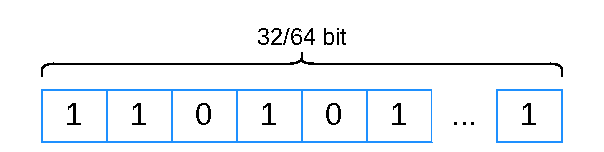
\includegraphics[width=0.7\linewidth]{logos/4_3cripto.pdf}
\end{figure}

Poi si scelgono dei \textbf{tap}, ovvero delle posizioni del buffer.  
Ad esempio, supponiamo di scegliere le posizioni \textbf{2}, \textbf{3} e \textbf{5}. Il numero di tap può variare.  
Queste posizioni saranno usate perché i bit in quelle posizioni verranno \textbf{xorati} tra loro; il risultato andrà in testa al registro e tutti i bit verranno spostati verso destra (e l'\textbf{ultimo} bit andrà perso).


Per esempio, supponiamo di avere un registro a 8 bit con il seguente stato iniziale:


\begin{figure}[h]
    \centering
    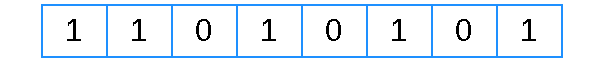
\includegraphics[width=0.7\linewidth]{logos/4_4cripto.pdf}
\end{figure}

Supponiamo che i \textbf{tap} siano: \textbf{2}, \textbf{3} e \textbf{5}.  
Allora, il numero successivo sarà dato dallo \textbf{xor} di questi tre bit.


\begin{center}
    nuovo bit = bit posizione 2 $\oplus$ bit posizione 3 $\oplus$ bit posizione 5 \\
    nuovo bit = 1 $\oplus$ 0 $\oplus$ 0 \\
    nuovo bit = 1
\end{center}

Ora, spostiamo tutti i bit di una posizione verso destra nel registro.


\begin{figure}[!h]
    \centering
    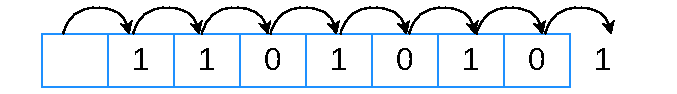
\includegraphics[width=0.7\linewidth]{logos/4_5cripto.pdf}
\end{figure}

Il bit che "sporge" a destra può essere escluso, e in prima posizione inseriamo il bit che abbiamo calcolato in precedenza.


\begin{figure}[!h]
    \centering
    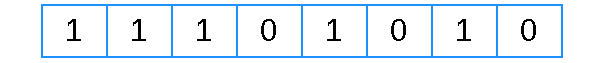
\includegraphics[width=0.7\linewidth]{logos/4_6cripto.pdf}
\end{figure}

E questo sarà il nuovo numero casuale, se ne volessi altri basta rieseguire il procedimento su questo nuovo stato del registro.

\newpage

Una cosa interessante è notare che i \textbf{tap} possono essere espressi come \textbf{polinomi}.  
Rimanendo con l'esempio di prima dei tap (\textbf{2}, \textbf{3}, \textbf{5}), possiamo esprimere questa configurazione tramite il seguente polinomio:


\begin{equation*}
    p(x) = x^2 + x^3 + x^5 +1
\end{equation*}

Qualsiasi configurazione è esprimibile tramite un polinomio, dove i gradi della variabile $x$ corrispondono ai tap, con l'aggiunta di un termine noto ($+1$), e tutti i monomi hanno coefficiente 1.


Questo polinomio ha permesso di studiare le configurazioni ottimali per ottenere una generazione di numeri migliore.  
Infatti, grazie alla rappresentazione polinomiale, si è scoperto che se il polinomio è \textbf{primitivo modulo 2}, la generazione di numeri pseudo-casuali sarà massima.  
Non entrerò nei dettagli, ma considerate che un polinomio primitivo modulo 2 è simile a un \textbf{numero primo}, nel senso che non esistono prodotti di polinomi modulo 2 che diano come risultato quel polinomio primitivo.


Per esempio, il polinomio $p(x) = x^2 + x + 1$ è primitivo, perché non può essere scritto come prodotto di altri polinomi.  
Invece, il polinomio $p(x) = x^2 + 1$ non è primitivo, perché, in modulo 2, può essere scritto come:


\begin{align*}
    p(x) &= (x+1)^2 \pmod{2} \\ 
         &= x^2 + 2x +1 \pmod{2} \\
         &= x^2 +1 \pmod{2}
\end{align*}

Inoltre, sempre con questo meccanismo, la generazione sarà massima anche quando le posizioni sono \textbf{numeri primi tra loro} e quando il \textbf{numero di posti è pari}.


Se non avete compreso bene questa parte, non preoccupatevi: il bello di questo concetto è vedere come una rappresentazione polinomiale di un sistema possa aiutare a migliorarlo e a massimizzarne l'efficienza.


Grazie a questi accorgimenti, si è scoperto che il polinomio più sicuro per un LFSR a 16 bit è:

\begin{equation*}
    p(x) = x^{11} +x^{13} + x^{14} + x^{16} +1
\end{equation*}

\newpage

\subsection{Stream} 

Fatta la premessa sui \textbf{PRNG}, capiamo cosa sono gli stream.  
Gli stream cercano di replicare la forza della cifratura \textbf{OTP}, che, come abbiamo già visto, è l'unico sistema teoricamente impossibile da decifrare.  
In pratica, gli stream utilizzano un algoritmo \textbf{PRNG}, come \textbf{LCG} o \textbf{LFSR} che abbiamo visto prima, e ogni lettera del messaggio viene cifrata tramite una \textbf{cifratura OTP} (cioè mediante un'operazione \textbf{XOR}) con uno dei numeri generati dal PRNG.

Quindi, per cifrare con gli stream, si inizia generando una sequenza di numeri:

\begin{figure}[h]
    \centering 
    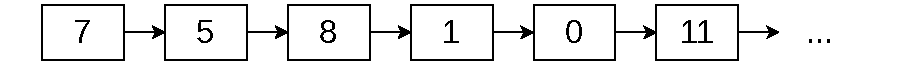
\includegraphics[width=0.8\linewidth]{logos/4_1cripto.pdf}
\end{figure}

Successivamente, ogni lettera del messaggio da cifrare viene combinata tramite un'operazione \textbf{XOR} con uno dei numeri generati.

\begin{figure}[h]
    \centering
    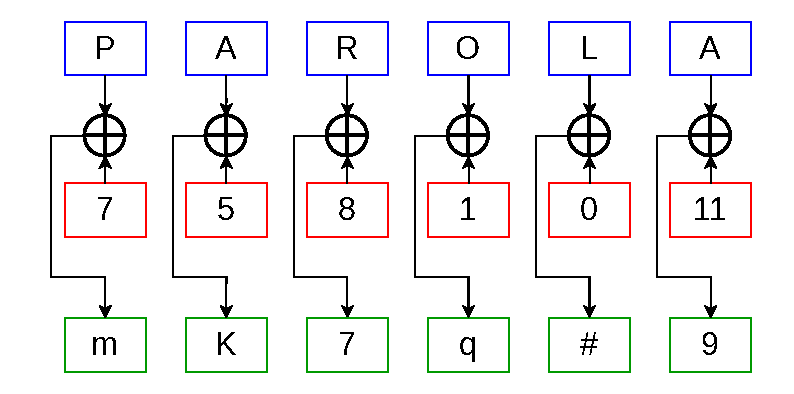
\includegraphics[width=0.8\linewidth]{logos/4_2cripto.pdf}
\end{figure}


\textbf{N.B.} Ricordo che il simbolo $\oplus$ indica l'operazione di \textbf{XOR}.


Cosi la stringa "\textbf{parola}" è diventata "\textbf{mK7q\#9}".

Per decifrarlo, sarà sufficiente rigenerare i numeri usando gli stessi parametri e lo stesso seed della cifratura; successivamente, basta eseguire nuovamente l'operazione \textbf{XOR} tra il messaggio cifrato e la chiave, proprio come avviene nella cifratura \textbf{OTP}.

La \textbf{chiave privata} di questo sistema è quindi il \textbf{seed} e i \textbf{parametri} del PRNG, perchè avendoli si può generare la sequenza di numeri e poi cifrare il messaggio. Anche se in realtà si possono rendere pubblici i parametri e lasciare \textbf{solamente il seed come chiave privata}, tanto con valori di paramentri molto altri (10/15 cifre) non rendono facilmente la rottura del cifrario


L'idea alla base degli stream è di replicare la sicurezza dell'\textbf{OTP} e di usare chiavi diverse per ogni cifratura, poiché ricordiamo che il problema dell'OTP è che non si può riutilizzare la stessa chiave, altrimenti si può risalire ai messaggi originali.


Ad oggi, però, i cifrari a \textbf{stream} non sono molto diffusi, a causa della difficoltà di generare numeri veramente casuali e perché, se si scopre il \textbf{seed} (che costituisce la chiave privata del cifrario), è possibile ricavare l'intero messaggio.


\end{document}